\documentclass[12pt]{article}
\usepackage[utf8]{inputenc}
\usepackage[T1]{fontenc}
\usepackage[francais]{babel}
\usepackage[usenames,dvipsnames]{xcolor}
\usepackage{listings}
\usepackage{amssymb}
\usepackage{amstext}
\usepackage{amsmath}
\usepackage[dvipsnames]{xcolor}
\usepackage{setspace}

%%novalidate

\usepackage{tikz}
\usepackage{calc}
\usepackage{booktabs}
%\usepackage{hyperref}

% colors
\definecolor{color1}{HTML}{000060}
%\definecolor{color1}{HTML}{8C260F}
\definecolor{color2}{HTML}{333333}
\definecolor{color_text}{HTML}{BBBBBB}
\definecolor{color_bg}{HTML}{2B2B2B}
\definecolor{color_comment}{HTML}{808080}

% fonts
\usepackage{fontspec}
\defaultfontfeatures{Mapping=tex-text}
\setmainfont
[Path = Fonts/,
BoldFont=Lato-Bold.ttf,
ItalicFont=Lato-Italic.ttf,
BoldItalicFont=Lato-BoldItalic.ttf]
{Lato-Regular.ttf}

%%%

\usepackage{geometry}
\geometry{a4paper,
hmargin=20mm,vmargin=20mm,
head=0ex,foot=3ex}

\linespread{1.3}

\usepackage[hang]{caption}
\DeclareCaptionFormat{upper}{#1#2\uppercase{#3}\par}
\captionsetup{labelfont={bf,color=color2},textfont={normalsize,color=color2},format = upper,figurename=FIGURE,tablename=TABLE}

%%% fancy sections
\usepackage{titlesec}
%\titleformat{\chapter}{\headingfont\LARGE\bfseries\scshape\color{color1}}{\thechapter}{1em}{}[\titlerule]
\titleformat{\section}{\color{color1}\headingfont\Large\bfseries\uppercase}{\thesection}{1em}{}[\titlerule]
\titleformat{\subsection}{\color{color1}\headingfont\large\bfseries}{\thesubsection}{1em}{}
\titleformat{\subsubsection}{\color{color1}\headingfont\bfseries}{\thesubsubsection}{1em}{}
%%%

% head and foot
\usepackage{fancyhdr}
\pagestyle{fancy}
\lhead{}
\chead{}
\makeatletter
\rhead{\color{color2} \today}
\makeatother
\newlength{\myheight}
\lfoot{
\settoheight{\myheight}{\thepage}
\raisebox{-2ex-0.5\myheight}{}
}
\cfoot{\color{color2}Méta-Heuristiques}
\rfoot{\color{color2}\thepage}
\renewcommand\headrulewidth{0pt}
\renewcommand\footrulewidth{0pt}


%%%
% custom titlepage
\usepackage{eso-pic}
\makeatletter
\renewcommand{\maketitle}{
\begingroup
\thispagestyle{empty}
\AddToShipoutPicture*{\put(0,0){
\includegraphics[width=\paperwidth,height=\paperheight,keepaspectratio]{Pictures/cover}}}  % Image background
\centering
\topskip0pt
\vspace*{\fill}
\par\normalfont\fontsize{35}{35}\sffamily\selectfont
\textbf{\color{color1}\@title}\\
{\LARGE \subtitle}\par % Book title
\vspace*{1cm}
\begin{spacing}{1.5}
{\Huge \@author}\par % Author name
\end{spacing}
\vspace*{\fill}
\endgroup
\clearpage
}
\makeatother

%%%


%%% fancy boxes
\usepackage{tcolorbox}
\usepackage{wrapfig}
\def\fullboxbegin{
\bigskip
\begin{tcolorbox}[colback=color1,colframe=color1,coltext=white,arc=0mm,boxrule=0pt]
}
\def\fullboxend{\end{tcolorbox}\medskip}
%
\def\leftboxbegin{
\begin{wrapfigure}{l}{0.5\textwidth}
\begin{tcolorbox}[colback=color1,colframe=color1,coltext=white,arc=0mm,boxrule=0pt]
}
\def\leftboxend{
\end{tcolorbox}
\end{wrapfigure}
}
%
\def\rightboxbegin{
\begin{wrapfigure}{r}{0.5\textwidth}
\begin{tcolorbox}[colback=color1,colframe=color1,coltext=white,arc=0mm,boxrule=0pt]
}
\def\rightboxend{
\end{tcolorbox}
\end{wrapfigure}
}
%
\newcounter{frames}
\def\frameboxbegin#1{
\bigskip
\refstepcounter{frames}
\begin{tcolorbox}[colback=white,colframe=color1,arc=0mm,title={\textbf{#1}}]
}
\def\frameboxend{
\end{tcolorbox}
}
%%%

\newtoggle{InString}{}% Keep track of if we are within a string
\togglefalse{InString}% Assume not initally in string

\lstset{
tabsize=2,
language=Python,
breaklines=true,
postbreak=\mbox{\textcolor{Gray}{$\hookrightarrow$}\space},
basicstyle=\ttfamily\footnotesize\color{color_text},
keywordstyle=\bfseries\color{Orange},
commentstyle=\color{color_comment},
morekeywords={assert},
keywords=[2]{self},
keywords=[3]{__init__},
keywords=[4]{None,True,False},
keywordstyle={[2]\ttfamily\color{Fuchsia}},
keywordstyle={[3]\ttfamily\color{Plum}},
keywordstyle={[4]\ttfamily\color{Periwinkle}},
showstringspaces=false,
backgroundcolor=\color{color_bg},
stringstyle=\color{SpringGreen}
}

\newtoggle{InString}{}% Keep track of if we are within a string
\togglefalse{InString}% Assume not initally in string

\begin{document}

\lstset{
tabsize=2,
language=Python,
breaklines=true,
postbreak=\mbox{\textcolor{Gray}{$\hookrightarrow$}\space},
basicstyle=\ttfamily\footnotesize\color{color_text},
keywordstyle=\bfseries\color{Orange},
commentstyle=\color{color_comment},
keywords=[2]{self},
keywords=[3]{__init__},
keywords=[4]{None,True,False},
keywordstyle={[2]\ttfamily\color{Fuchsia}},
keywordstyle={[3]\ttfamily\color{Plum}},
keywordstyle={[4]\ttfamily\color{Periwinkle}},
showstringspaces=false,
backgroundcolor=\color{color_bg},
stringstyle=\color{SpringGreen}
}


%----------------------------------------------------------------------------------------
%	TITLE
%----------------------------------------------------------------------------------------

\title{Méta-Heuristiques}
\def\subtitle{Flexible Job Shop Scheduling Problem}
\author{Samy Barrech \\ Jonathan Poncy}

\maketitle

%----------------------------------------------------------------------------------------
%	TABLE OF CONTENTS
%----------------------------------------------------------------------------------------

\tableofcontents % Print the table of contents itself
\clearpage

%----------------------------------------------------------------------------------------
%	CHAPTER 1
%----------------------------------------------------------------------------------------

\section{Introduction}

\subsection{Présentation du projet}

Dans ce projet, nous considérons un problème d'ordonnancement appelé "Flexible Job Shop". Nous disposons d'un ensemble de $n$ travaux (jobs) devant être exécutés sur $m$ machines. Chaque job se décompose en une liste d'activités qui doivent être réalisées dans l'ordre. Une activité est décrite par un ensemble d'opération de durée et de machine différente et il faut choisir l'opération qui minimise la durée totale que nécessite l'ensemble des jobs pour être terminé.

On supposera que les machines ne peuvent réaliser qu'une opération à la fois bien que la solution que nous proposons dans le cas d'une recherche à l'aide d'une heuristique, les machines peuvent supporter plusieurs opérations en simultané. Dans le cas de l'approche génétique, ce nombre est fixé à une seule opération en simultané.

\subsection{Structure des jeux de données}

Voici un exemple de jeu de données:
\lstinputlisting[xleftmargin=2cm,backgroundcolor=\color{white},basicstyle=\ttfamily\footnotesize\color{black}]{./app/data/test.fjs}

La première ligne représente le nombre de jobs, le nombre de machines et enfin le nombre d'opérations que la machine peut réaliser en parallèle. Ensuite, on retrouve une ligne par job. Le premier nombre de la ligne représente le nombre d'activités pour ce job. Le second (que l'on va appeler $k \geq 1$) correspond à la liste des opérations que l'on peut choisir pour réaliser l'activité. On retrouve ensuite $k$ paires correspondant au numéro de la machine et à la durée que prend l'opération, puis les données pour la seconde activité, etc. 

\subsection{Structure de notre projet}

Le code des classes se retrouvent dans les fichiers "job.py", "activity.py", "opertion.py" et "machine.py". Nous ne rentrerons pas dans le détail de ces derniers, le code étant suffisament explicite.

\subsubsection{Classe représentant les jobs}

Un Job se décompose comme un identifiant, la liste des activités à réaliser et la liste des activités déjà réalisées.

\subsubsection{Classe représentant les activités}

Une activité est composée d'un pointeur vers le job auquel elle est rattachée, d'un identifiant d'activité, de la liste des opérations possible et de l'opération réalisée.

\subsubsection{Classe représentant les opérations}

Une opération est décrite par un identifiant, une durée, l'identifiant de la machine qui doit procéder à l'opération, l'instant $t$ où l'opération est commencée, un ordre d'arrivée dans la machine (utile pour dessiner le planning), et d'un booléen pour indiquer si l'opération est en cours de traitement.

\subsubsection{Classe représentant les machines}

\newpage

%----------------------------------------------------------------------------------------
%	CHAPTER 2
%----------------------------------------------------------------------------------------

\section{Résolution à l'aide d'une heuristique}

\subsection{Objectifs de la méthode}

Cette méthode permet de trouver une borne supérieure de l'optimum très rapidement. Elle consiste à appliquer une heuristique au moment de choisir quelles opérations les machines vont traiter.

\subsection{Algorithme du scheduler}

\subsubsection{Instanciation de la classe, paramètres de la méthode et initialisation}

\lstinputlisting[firstline=7, lastline=14]{./app/scheduler.py}

Le constructeur de la classe prend trois paramètres, la liste des machines, le nombre maximal d'opérations en parallèle et la liste des jobs construite avec le parseur. La variable \textit{original\_stdout} permet de supprimer la sortie texte et de la rétablir au besoin.

\begin{lstlisting}
s = Scheduler(machines_list, number_max_operations, jobs_list)
\end{lstlisting}

Pour démarrer le scheduler, il suffit d'appeler la méthode \textit{run} en passant en paramètre l'heuristique considérée et optionnelement mettre \textit{verbose} à \textit{True} ou \textit{False} en fonction de si l'on veut un affichage ou non.
\begin{lstlisting}
s.run(Heuristics.select_first_operation)
\end{lstlisting}

Lors de cet appel, la méthode \textit{run} va commencer par supprimer la sortie standard si nécessaire et initialiser la variable \textit{current\_step} à $0$. Cette variable représente l'instant $t$ dans lequel le système se trouve. 

\lstinputlisting[firstline=16, lastline=22]{./app/scheduler.py}

\newpage

\subsubsection{Déroulement de l'algorithme}

\lstinputlisting[firstline=24, lastline=42]{./app/scheduler.py}

La variable \textit{best\_candidates} correspond au retour de l'heuristique considérée. Il s'agit d'un dictionnaire associant aux identifiants des machines la liste des opérations (ainsi que l'activité auxquelle elles sont rattachées) qu'elles devraient traiter à l'instant $t$.

La boucle \textit{for} parcourant \textit{best\_candidates.items()} permet d'affecter l'opération sur la bonne machine.

La boucle \textit{for} parcourant \textit{self.\_\_machines} permet de simuler le travail des machines pendant une unité de temps.

\subsubsection{Fin de la méthode \textit{run}}

\lstinputlisting[firstline=44, lastline=50]{./app/scheduler.py}

On affiche la durée totale que le planning prend et on réactive \textit{std\_out} si nécessaire. 

\newpage

\subsection{Choisir l'opération la plus courte dans une activité comme heuristique}

\lstinputlisting[firstline=4, lastline=5]{./app/heuristics.py}

Lors de l'appel de cette heuristique, le paramètre de temps n'est pas utile, d'où la wild card utilisée et on commence par initialiser le dictionnaire \textit{best\_candidates}.

\lstinputlisting[firstline=7, lastline=27]{./app/heuristics.py}

Ensuite, pour chaque job qu'il reste à faire, on récupère l'activité en cours. Ici, on considère que la meilleure opération à choisir est celle qui a la durée la plus courte. On met à jour le dictionnaire en fonction de son état :
\begin{itemize}
    \item Si la machine n'a aucune opération affectée, on ajoute la machine au dictionnaire avec l'activité et l'opération calculée précédemment.
    \item Si la machine a déjà des opérations affectées mais qu'elle ne travaille pas à capacité maximale, on ajoute l'activité et l'opération calculée précédemment à la liste
    \item Si la machine travaille à capacité maximale, on regarde s'il existe une opération de durée supérieure à celle calculée précédemment et si c'est le cas, on la remplace.
\end{itemize}

\lstinputlisting[firstline=29, lastline=29]{./app/heuristics.py}

Enfin, on renvoie le dictionnaire calculé.
\newpage

%----------------------------------------------------------------------------------------
%	CHAPTER 3
%----------------------------------------------------------------------------------------

\section{Approche génétique}

\subsection{Que sont les algorithmes génétiques ?}

Les algorithmes génétiques sont des méthodes évolutionnistes qui simulent une évolution naturelle, génération après génération, où les individus peuvent muter, se croiser ou se reproduire (cloner).

Ils permettent, lorsqu'il n'existe pas de méthode exacte (ou que la solution est inconnue), d'obtenir une solution approchée en un temps raisonnable.

Dans ce projet, nous nous basons sur une librairie Python qui s'appelle \textit{Deap}.

\subsection{Instanciation de la classe et lancement de la méthode}

\begin{lstlisting}
s = GeneticScheduler(machines_list, jobs_list)
\end{lstlisting}

Le constructeur de la classe prend comme arguments la liste des machines et la liste des jobs que renvoie le parseur.

\begin{lstlisting}
s.run_genetic(total_population=10, max_generation=100, verbose=True)
\end{lstlisting}

Pour lancer l'algorithme, la métode \textit{run\_genetic} prend comme paramètres le nombre total d'individus dans la population, la génération maximale et si l'utilisateur souhaite activer la sortie standard ou non. Tous ces paramètres sont facultatifs et valent respectivement $10$, $100$ et \textit{True} par défaut.

\subsection{Création d'un individu}

\lstinputlisting[firstline=38, lastline=42]{./app/geneticscheduler.py}

Afin de trouver un individu initial, nous réalisons une copie profonde de la liste des jobs et des machines. En effet, ces dernières seront modifiées par le \textit{scheduler} de la partie précédente ce qui empêcherait toute autre simulation par la suite.

\lstinputlisting[firstline=44, lastline=47]{./app/geneticscheduler.py}

Le \textit{scheduler} est ensuite appelé sur les listes temporaires précédemment créer.

\lstinputlisting[firstline=49, lastline=55]{./app/geneticscheduler.py}

Comme l'opération a été réalisée sur des listes temporaires, il est nécessaire de faire la correspondance des activités et des opérations sur les listes initiales, les objets étant différents. Les couples \textit{activity} et \textit{operation} sont ensuite stockées dans une liste avec le temps auquel l'opération commence afin de pouvoir trier cette liste pour respecter la contrainte d'ordre.

\lstinputlisting[firstline=56, lastline=60]{./app/geneticscheduler.py}

La liste est donc triée par rapport au temps, puis on supprime cette composante de la liste pour créer notre individu. Les variables temporaires sont détruites et l'individu retourné.

\subsection{Création de la population initiale}

\lstinputlisting[firstline=62, lastline=65]{./app/geneticscheduler.py}

Notre population initiale correspond à $total\_population$ éléments. Chaque élement correspond à l'individu retourné par la méthode \textit{init\_individual}.

\subsection{Evaluation de la fonction objectif d'un individu}

\lstinputlisting[firstline=114, lastline=115]{./app/geneticscheduler.py}

L'évaluation d'un individu est très simple. Comme nous souhaitons minimiser le temps total que mettent les jobs, l'évaluation correspond logiquement au temps que met l'individu pour terminer. Cette évaluation fait donc appel à la méthode \textit{compute\_time}. 
\newpage

Cette évaluation repose sur une astuce. Comme les activités sont classées par ordre chronologique, il suffit de regarder à quel instant $t_1$ termine l'activité précédente du job et à quel instant $t_2$ termine la dernière activité sur la machine concernée par l'opération couramment considérée. Il suffit ensuite de prendre le max entre $t_1$ et $t_2$ pour avoir l'instant $t$ auquel l'activité commence.

\lstinputlisting[firstline=67, lastline=78]{./app/geneticscheduler.py}

On initialise une liste contenant pour chaque activité le temps auxquel elles commencent (utile pour la simulation finale) et deux dictionnaires, un premier faisant la correspondance entre $machine\_id$ et liste des opérations réalisées par cette mmachine, le deuxième faisant la même chose mais par rapport aux identifiants des jobs.

\lstinputlisting[firstline=80, lastline=101]{./app/geneticscheduler.py}

On calcule ensuite les instants de temps comme indiqué précédemment.

\lstinputlisting[firstline=103, lastline=111]{./app/geneticscheduler.py}

Pour calculer le temps total que prend le planning, on regarde pour chaque machine le moment où la dernière opération commence ainsi que sa durée et on prend la somme maximale. Enfin, on renvoie la durée totale et la liste des instants temporels.

\subsection{Mutation d'un individu}

\lstinputlisting[firstline=120, lastline=123]{./app/geneticscheduler.py}

Pour réaliser la mutation d'un individu, on commence par faire une copie profonde de ce dernier et on regarde les activités qui peuvent muter, autrement dit celles où plusieurs opérations sont possibles pour les réaliser.

\lstinputlisting[firstline=124, lastline=132]{./app/geneticscheduler.py}

S'il existe de telles activités, on en choisit une au hasard, et pour cette activité on choisit une opération différente. 

\lstinputlisting[firstline=133, lastline=136]{./app/geneticscheduler.py}

On supprime la composante \textit{fitness} (qui correspond à la fonction objective) car sa valeur n'est plus à jour et on renvoie le mutant.

\subsection{Permutation sur un individu}

Une permutation sur un individu correspond à une permutation de deux couples activité/opération ne violant pas la contrainte d'ordre. 

Exemple de planning en identifiant les activités par \textit{(id\_job, id\_activity)}:

\begin{figure}[!h]
    \centering
    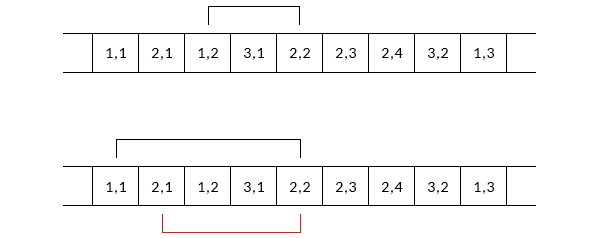
\includegraphics[scale=0.8]{report/Pictures/permutation.png}
\end{figure}

Par exemple, la première permutation est valide car elle respecte la contrainte d'ordre. Cependant, pour la deuxième, la contrainte d'ordre ne serait plus respectée car si j'échange le $(1,1)$ et le $(2,2)$, alors on aurait $(2,2)$ avant $(2,1)$ ce qui est impossible, de même avec $(1,1)$ et $(1,2)$. 

\lstinputlisting[firstline=143, lastline=155]{./app/geneticscheduler.py}

\newpage

Cette méthode permet de calculer les bornes min et max de permutation pour une activité donnée, autrement dit l'intervalle où l'on peut déplacer une activité sans que cela viole la contrainte d'ordre.

\lstinputlisting[firstline=157, lastline=179]{./app/geneticscheduler.py}

On réalise dans un premier temps une copie profonde de l'individu. Ensuite, tant que l'on a pas trouvé une permutation possible, on sélectionne deux activités au hasard et on vérifie si elles sont permutables, c'est à dire si chacune appartient au domaine de permutation de l'autre. Une fois cette permutation trouvée, elle est effectuée et le nouvel individu est renvoyé.

Il est a noté qu'une permutation est forcément possible à partir du moment où le nombre de jobs est au moins égal à deux.

\newpage

\subsection{Evolution d'un individu}

\lstinputlisting[firstline=182, lastline=188]{./app/geneticscheduler.py}

Un individu donné peut muté, subir une permutation, ou les deux. On calcule pour cela deux probabilités, une par opération possible. Bien que par construction ces opérations respectent forcément la contrainte d'ordre, on effectue une vérification sur le futur individu.

\subsection{Simulation sur les machines d'un individu}

\lstinputlisting[firstline=190, lastline=198]{./app/geneticscheduler.py}

Pour un individu donné, on simule son exécution afin de pouvoir le dessiner éventuellement.

\subsection{Déroulement de l'algorithme}

\lstinputlisting[firstline=201, lastline=212]{./app/geneticscheduler.py}

Lors de l'appel de la méthode \textit{run\_genetic}, on commence par désactiver la sortie standard si demandé puis on initialise la libraire \textit{Deap}. On indique que l'on chercher à minimiser la fonction objectif. On enregistre également auprès de \textit{Deap} nos fonctions de création, de mutation, de permutation et d'évolution.

\lstinputlisting[firstline=214, lastline=215]{./app/geneticscheduler.py}

On crée ensuite notre population initiale.

\lstinputlisting[firstline=217, lastline=237]{./app/geneticscheduler.py}

On simule l'évolution pour $max\_generation$ générations. On définit les probabilités de mutations et de permutation puis on fait évoluer notre population et enfin on évalue la fonction objectif de chaque individu. Si un individu a une fonction objectif plus faible que \textit{best}, alors cet individu devient le meilleur individu. De plus, pour augmenter l'efficacité de notre algorithme vers la convergence de l'optimum, nous avons décidé de remplacer la population actuelle par une population composée uniquement du meilleur individu.

\newpage

\lstinputlisting[firstline=239, lastline=251]{./app/geneticscheduler.py}

On affiche les résultats et on simule le meilleur planning trouvé. On réactive la sortie standard si besoin.
\newpage

%----------------------------------------------------------------------------------------
%	CHAPTER 4
%----------------------------------------------------------------------------------------

\section{Résultats et comparaison des méthodes}

\subsection{Résultats avec un jeu de données simple}

\begin{figure}[!h]
    \centering
    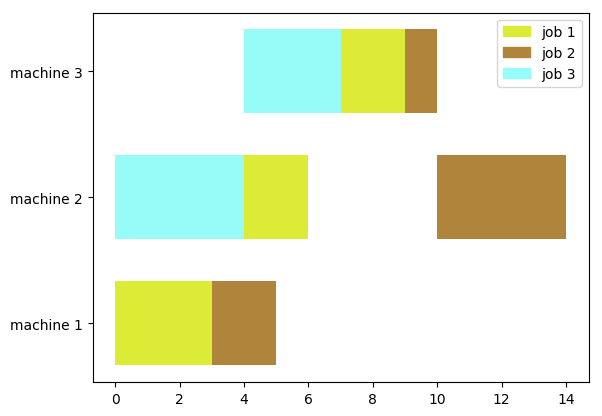
\includegraphics[]{results/test_shortest_operation.png}
\end{figure}

\begin{figure}[!h]
    \centering
    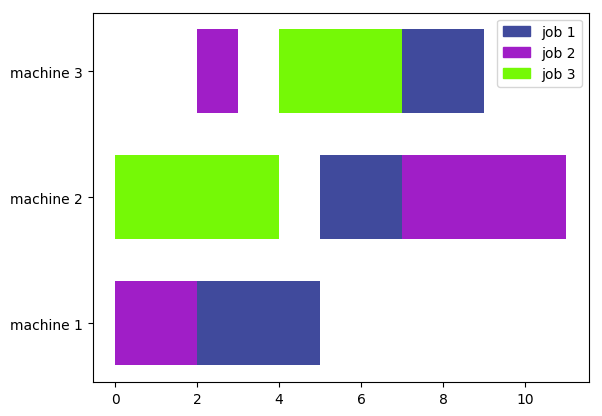
\includegraphics[]{results/test_genetic.png}
\end{figure}

\subsection{Barnes - setb4c9}

\begin{figure}[!h]
    \centering
    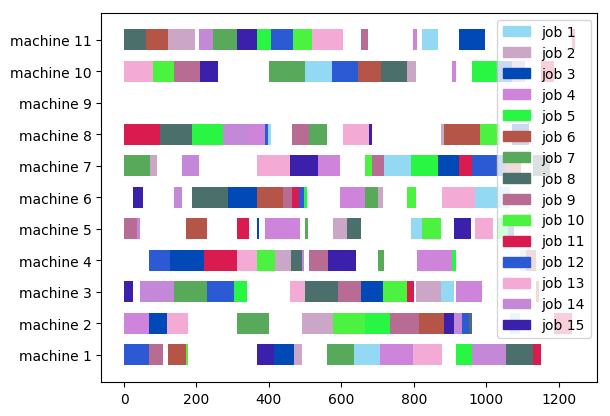
\includegraphics[]{results/barnes_setb4c9_shortest_operation.png}
\end{figure}

\begin{figure}[!h]
    \centering
    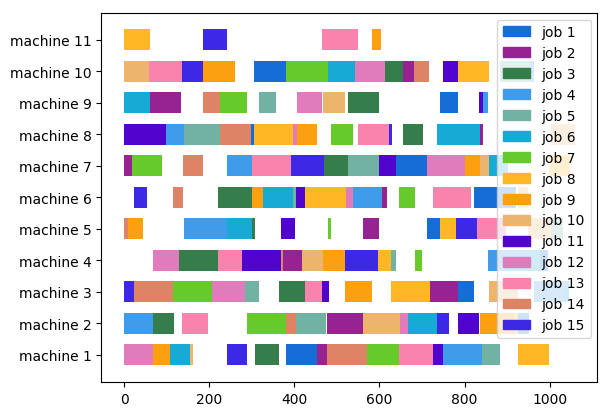
\includegraphics[]{results/barnes_setb4c9_genetic.png}
\end{figure}




\end{document}          
